\chapter{Arquitectura}
\label{Arquitectura}
Este apartado describe la arquitectura software de \textbf{Virus Breaker}. La descripción comenzará con una recapitulación de los eventos con los que un jugador se encontrará cuando inicie una sesión de juego. A esta descripción le seguirá a un análisis técnico de la estructura interna del juego, comenzando por las \textbf{escenas} en las que este se divide y terminando con un análisis de cada uno de los \textbf{objetos} que intervienen en el desarrollo de la acción.

\section{Descripción del Juego}
Como programa informático, Virus Breaker constara de un \textbf{archivo ejecutable}, acompañado de una carpeta que almacena ficheros complementarios. Para iniciar el juego, el jugador deberá simplemente iniciar el archivo ejecutable, sin necesidad de ningún tipo de instalación previa.

Una vez iniciado, el juego presentará al jugador una sencilla \textbf{pantalla de titulo}. La funcionalidad de esta pantalla será limitada, solo mostrará el título y el nombre del desarrollador del juego; e informará al jugador de que botón debe pulsar para iniciar una partida. En la figura \ref{titulo} se puede ver la apariencia de esta pantalla de título en la versión final del juego.
\begin{figure}[h]
    \centering
    \label{titulo}
    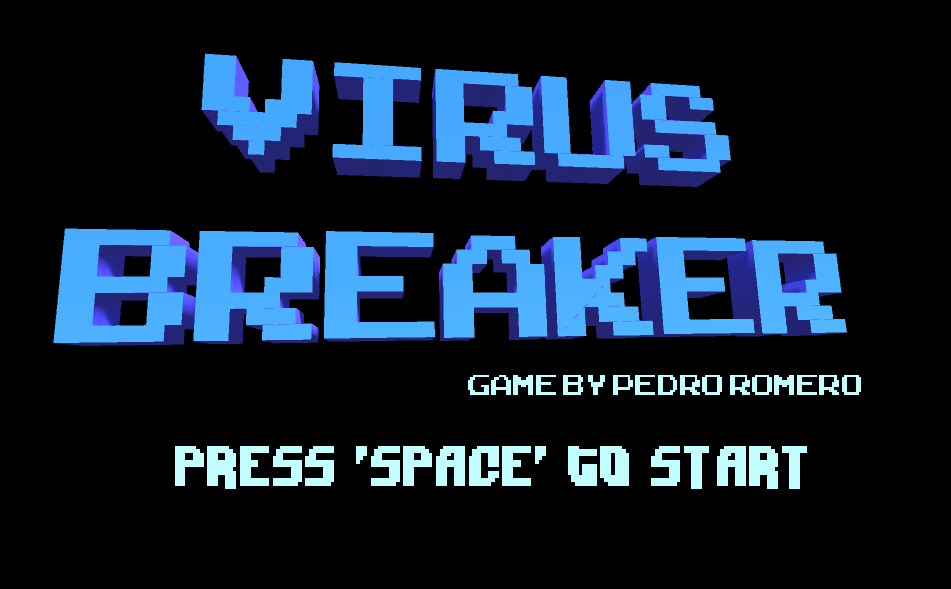
\includegraphics[width=0.6\textwidth]{images/estructura/escenas/titulo}
    \caption{Pantalla de título.}
\end{figure}

Una vez iniciada la partida, el jugador pasará a controlar al \textbf{personaje principal} e intentará superar los desafíos que le presente el juego. Una versión básica de esta pantalla se puede ver en la figura \ref{juego}. El juego se dividirá en varios \textbf{niveles}, cada vez que el jugador supere uno, el juego le presentará otro de dificultad mayor. Esta secuencia de niveles concluirá con el enfrentamiento contra un \textbf{Jefe Final}. Al derrotar al jefe final, el juego mostrara una \textbf{pantalla de victoria}. Esta pantalla será funcionalmente idéntica a la pantalla de título: mostrara un mensaje y permitirá al jugador volver a jugar al juego si pulsa un botón. 

\begin{figure}[h]
    \centering
    \label{juego}
    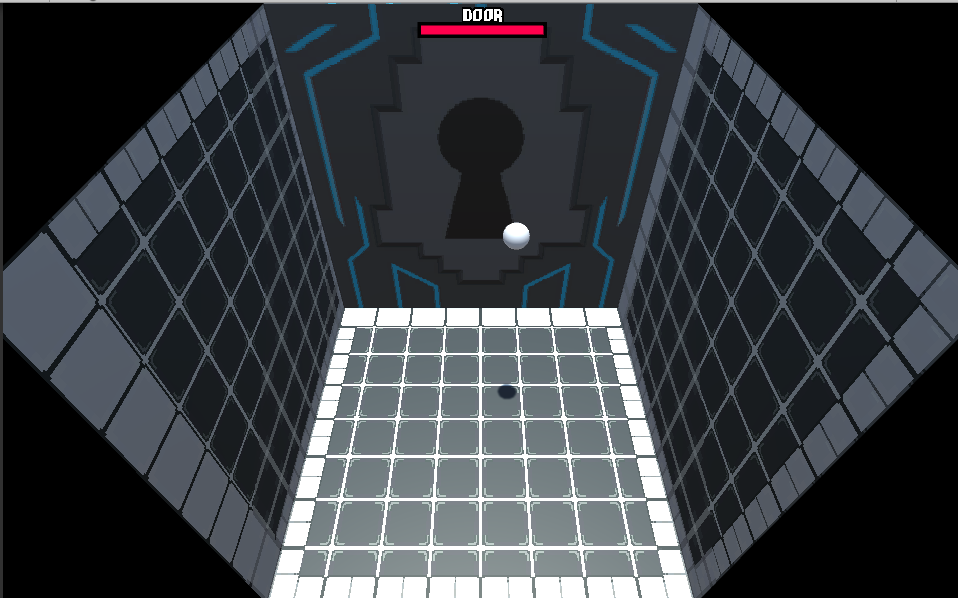
\includegraphics[width=0.6\textwidth]{images/estructura/escenas/juego}
    \caption{Pantalla de juego.}
\end{figure}

Si el jugador es derrotado durante el juego, se le mostrará una pantalla de \textbf{fin del juego}, donde se le ofrecerá la posibilidad de volver a iniciar la partida desde el ultimo nivel superado. A igual que la pantalla de victoria, la funcionalidad de esta pantalla será idéntica a la de la pantalla de título. La similitud entre estas tres pantallas se puede apreciar en la figura \ref{win_lose}

\begin{figure}[h]
    \centering
    \label{win_lose}
    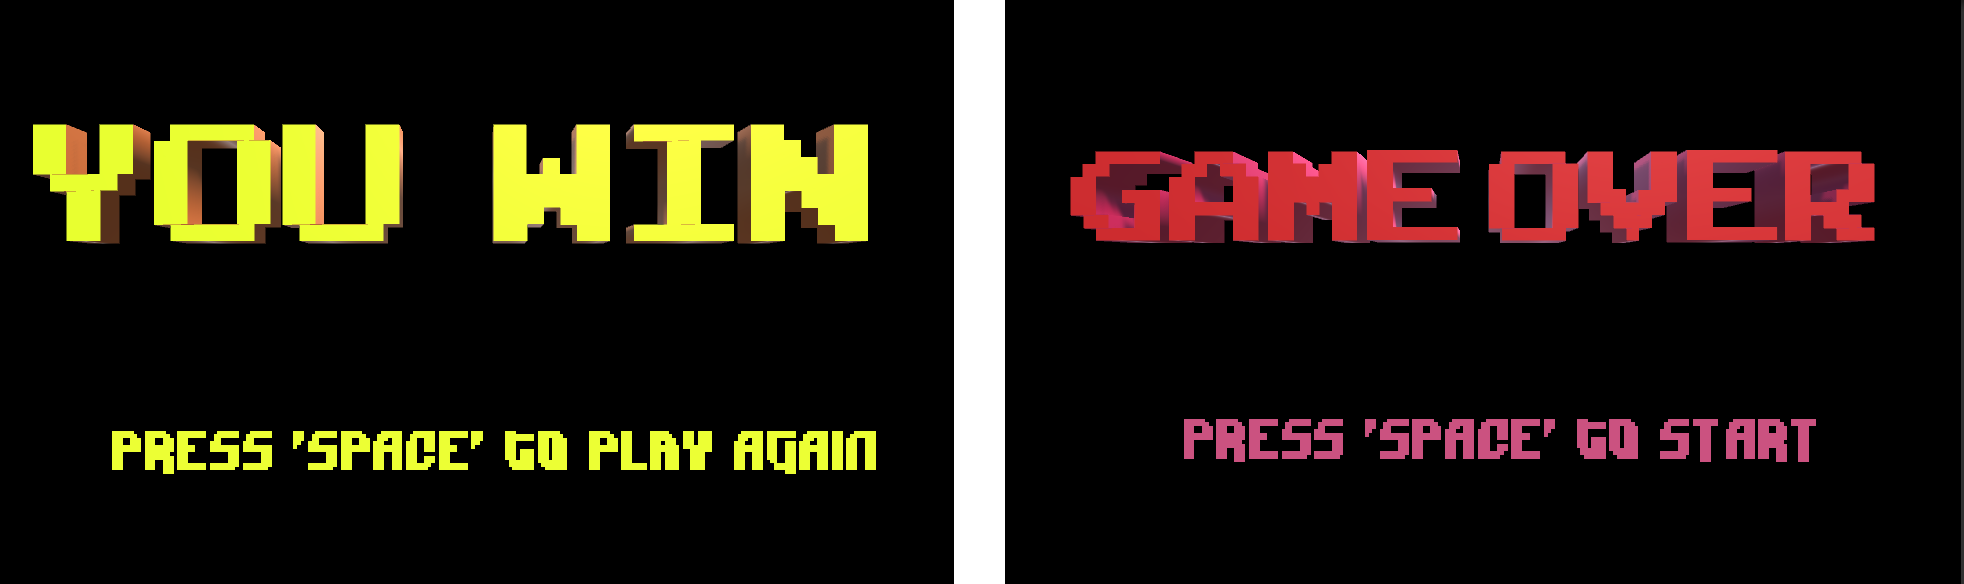
\includegraphics[width=0.6\textwidth]{images/estructura/escenas/win_lose}
    \caption{Pantallas de victoria y derrota.}
\end{figure}

El progreso del jugador en el juego se guarda entre partidas, de forma que si el juego se cierra, el jugador pueda empezar por el mismo nivel en el que se encontraba la siguiente vez que inicie el juego. Cuando se derrota al jefe final, la partida guardada se elimina para permitir que el jugador pueda volver a jugar desde el principio si lo desea.

\section{Escenas}
Desde un punto de vista formal, este juego, al igual que el resto de juegos, es una \textbf{aplicación gráfica interactiva} con renderizado en tiempo real \cite{libro_esi}. Este tipo de aplicaciones están construidas sobre un bucle de ejecución (llamado comúnmente \textbf{bucle de juego} en el ámbito del videojuego) el cual esta formado por tres pasos:
\begin{enumerate}
\item \textbf{Renderizar} una imagen a traves de la pantalla del usuario.
\item \textbf{Leer} la entrada que el usuario suministre.
\item \textbf{Modificar} el estado del programa, del cual depende la siguiente renderización.
\end{enumerate}
Cuando se trata de un videojuego, este sistema de renderizado es acompañado de sistemas de audio, simuladores de físicas y otros subsistemas que permita dotar al jugo de realismo e inmersividad.

En la gran mayoría de los videojuegos se pueden distinguir una serie de ``etapas'' o ``estados'', en cada uno de los cuales se ejecuta una lógica distinta independiente. En nuestro caso, cada una de las ``pantallas'' descritas en el apartado anterior serían uno de estos estados. La mayor parte de los motores de juego permiten e incluso fomentan que programador realice estas divisiones del juego ofreciendo implementaciones de estos estados. dependiendo del motor, estas divisiones se pueden llamar \textbf{salas, mundos o escenas}.

En Unity, los estados del juego reciben el nombre de \textbf{Escena} \footnote{https://docs.unity3d.com/Manual/CreatingScenes.html}. A grandes rasgos, las escenas son un conjunto de entidades de juego situadas en un entorno tridimensional. Estas entidades se encuentran organizadas en un \textbf{grafos de escena}, un tipo de estructura de datos que permite representar las relaciones jerárquicas que existen entre los distintos objetos del juego o ``nodos'' haciendo uso de un grafo dirigido sin hijos \cite{libro_esi}. El uso de este tipo de estructura permite gestionar con facilidad escenas tridimensionales complejas, permitiendo que se apliquen las operaciones transformaciones (como la traslación, rotación y escalado) de un nodo padre a todos sus nodos hijos de forma automática y facilita tareas como las búsquedas de entidades concretas.

\begin{figure}[h]
    \centering
    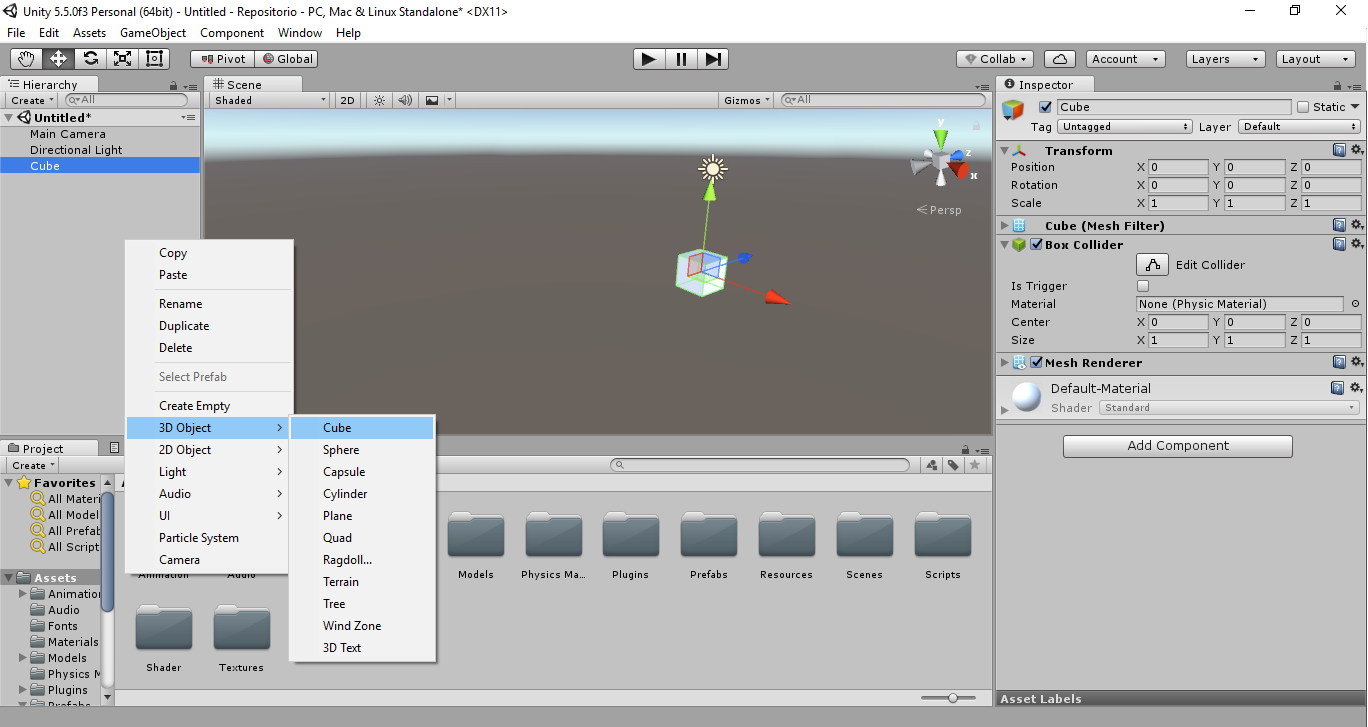
\includegraphics[width=0.8\textwidth]{images/estructura/escenas/editor}
    \caption{Editor de escenas de Unity.}
    \label{scene_editor}
\end{figure}

La suite de desarrollo de Unity incluye un editor de escenas, que permite la creación de estas mediante una interfaz gráfica. Las escenas se almacenan en archivos, de la misma forma que lo hacen las texturas o los modelos 3D, lo que facilita su gestión. Para la manipulación de escenas en tiempo de ejecución se utiliza el módulo \textbf{SceneManager} \footnote{https://docs.unity3d.com/ScriptReference/SceneManagement.SceneManager.html} que permite realizar cambios de escenas, cargar escenas en segundo plano y solapar varias escenas simultáneamente entre otras funciones. 

Para Virus Breaker, se optó por una estructura en cuatro Escenas: tres escenas de ``menú'' (menú de inicio, fin del juego y victoria) y una escena de juego, como puede verse en la figura \ref{scenes}. A continuación, se realizará una descripción de estos tipos de escenas

\begin{figure}[h]
	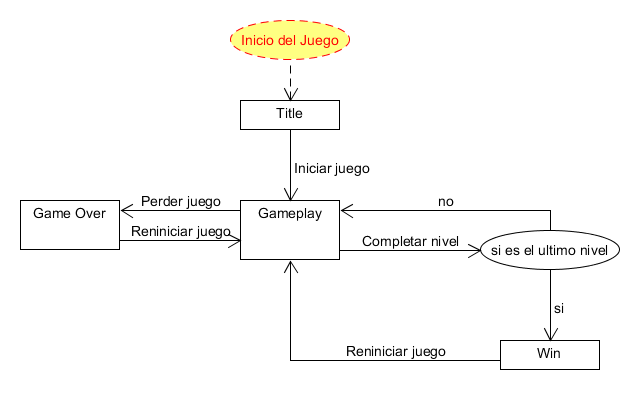
\includegraphics[width=0.8\textwidth]{images/estructura/escenas/scenes}
	\centering
	\caption{Diagrama de las escenas del juego}
	\label{scenes}
\end{figure}

\subsection{Menus}
En el campo de la informatica, un \textbf{menú} es un tipo de interfaz de usuario en la que se presenta una lista de elementos (que pueden ser comandos, opciones o atributos) de entre los cuales el usuario puede elegir \cite{apple_ui}. Su principal ventaja frente a otras alternativas (como el control por línea de comandos) radica en que el usuario \textbf{no necesita aprender de memoria todas las opciones} del menú para utilizarlo. En los videojuegos, la función de los menús suele ser la de contener las acciones necesarias para la ejecución del juego, pero que no pertenecen a la jugabilidad. Estas pueden ser guardar y cargar partidas, cambiar la configuración técnica del juego o elegir entre distintos modos de juego.

En Virus Breaker contamos con tres escenas que podrían considerarse menús: la \textbf{pantalla de título}, la \textbf{pantalla de victoria} y la \textbf{pantalla de derrota}. El comportamiento del juego en estas tres pantallas es prácticamente idéntico: El juego muestra un texto animado de gran tamaño, acompañado de un segundo texto con instrucciones para el jugador. Si el jugador pulsa el botón que aparece en las instrucciones, la escena cambiará a la escena de juego.

La animación de los textos se realizó mediante \textbf{Mecanim}\footnote{https://docs.unity3d.com/462/Documentation/Manual/MecanimAnimationSystem.html}, el sistema de animaciones integrado de Unity, que permite realizar cambios en parámetros de objetos de juego en función del tiempo. Los textos pequeños fueron creados también en Unity, pero los textos grandes fueron modelados en \textbf{Blender}\footnote{https://www.blender.org/} y luego importados en Unity.

El código que controla los menús es realmente simple, un pequeño script en C\# revisa si el jugador a pulsado la tecla correspondiente y cuando esto pasa llama al gestor de escenas de Unity para cargar la escena de juego.

\subsection{Escena de Juego}
La escena de juego es en la que ocurre \textbf{la acción del juego}, donde el jugador controla el personaje principal intentando completar los distintos niveles del juego. Como puede verse en el diagrama \ref{scenes}, se trata de la escena central del juego, a donde se dirigen el resto de las escenas. 

Se trata por tanto de \textbf{la escena más compleja del juego}, la que tiene mayor número de elementos e interacciones y en la que más tiempo pasa el jugador durante su partida. En la figura \ref{juego_detalles} se pueden ver detallados los distintos elementos de alto nivel que tiene esta escena:

\begin{figure}[h]
	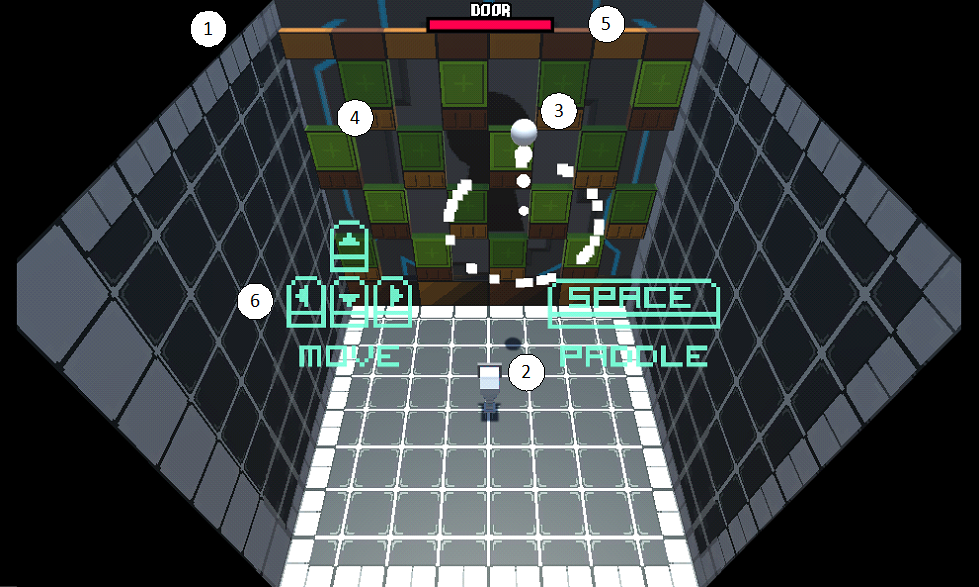
\includegraphics[width=0.8\textwidth]{images/estructura/escenas/juego_detalles}
	\centering
	\caption{Diagrama de las escenas del juego}
	\label{juego_detalles}
\end{figure}

\begin{enumerate}
\item\textbf{Sala}: La sala es el entorno en el que ocurre la partida. Está compuesta de tres paredes, suelo, techo y una puerta. La sala lleva el control del comportamiento general de la partida, encargándose de tareas como realizar transiciones de salas o activar y desactivar otros elementos según sea necesario.
\item\textbf{Personaje Principal}: Es el elemento sobre el que el jugador tiene un control directo. Puede moverse y crear una paleta. Su comportamiento se basa en una máquina de estados finitos.
\item\textbf{Pelota}: La pelota es un objeto que se mueve por la sala rebotando en sus paredes. Es posible el elemento más importante de la sala, ya que la mayor parta de interacciones entre objetos se realizan a través de la pelota
\item\textbf{Ladrillos}: Los ladrillos son unos elementos destructibles los cuales forman un muro que protege la puerta. Hay distintos tipos de ladrillos, cada uno con un comportamiento distinto.
\item\textbf{Resistencia de la puerta}: Se trata de una imagen que representa cuantos golpes necesita la puerta para abrirse.
\item\textbf{Tutorial en pantalla}: Son dos imágenes que muestran los controles del juego. Solo aparecen la primera vez que se inicia una partida, para no sobrecargar al jugador con información.
\end{enumerate}

\subsubsection{Carga de Niveles}
\label{level_generator}
Este juego cuenta con varios niveles, cada uno con una configuración de ladrillos distinta. Dado el gran número de elementos comunes que existen entre los distintos niveles (la geometría de la sala, el personaje, la pelota, la puerta...), utilizar una sala distinta por cada uno de los niveles \textbf{supondría un gasto innecesario de recursos} y generaría problemas a la hora de realizar \textbf{modificaciones sobre los elementos comunes}, cuyos cambios tendrían que propagarse manualmente en todos los niveles.

Para paliar con estos problemas, se optó por utilizar un editor externo para producir los niveles. Los niveles se \textbf{almacenarían en forma de archivos} que la escena se encargaría de leer para generar las formaciones de ladrillos correspondientes. La funcionalidad que se necesitaba para el editor de niveles era la siguiente:
\begin{itemize}
  \item \textbf{Precisión} a la hora de colocar y alinear los bloques. El editor debe ser capaz de posicionar los ladrillos en una cuadricula de forma automática (para así mantener la estética de juego deseada).
  \item Posibilidad de elegir individualmente el \textbf{color} para cada uno de los bloques del nivel, independientemente de su comportamiento o posición. Esto permite crear dibujos con los bloques, lo que hace los niveles más memorables (ejemplo en la figura \ref{ejemplo-arkanoid}). 
  \item \textbf{Simplicidad} en el proceso de creación. La creación de niveles debe de ser rápida, para facilitar la iteración el diseño.
\end{itemize}

\begin{figure}[h]
	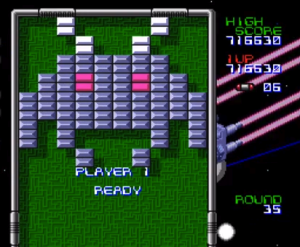
\includegraphics[width=0.7\textwidth]{images/estructura/niveles/ejemplo-arkanoid}
	\centering
	\caption{Homenaje a Space Invaders(Taito, 1978) dentro de Arkanoid: Doh it Again (Taito, 1997)}
	\label{ejemplo-arkanoid}
\end{figure}

En una primera versión, se planteó el uso del programa \textbf{Tiled}\footnote{http://www.mapeditor.org/}, un editor de mapas de propósito general que permite la edición de mapas basados en baldosas o \textbf{``tiles''} utilizando un sencillo procesador del lenguaje. Los mapas desarrollados generados con tiles eran exportados al formato \textbf{XML}, el cual podía se cargado en Unity. Sin embargo, al ser un programa de propósito general, Tiled contaba con mucha funcionalidad innecesaria que ralentizaba la producción de niveles, al mismo tiempo que carecía de ciertas funciones clave (como la selección individual de colores de bloques).

En la iteración final, se optó por almacenar la información de los niveles en forma de imágenes. Este nuevo sistema lee \textbf{pequeñas imágenes} que contienen la información del nivel codificada en los colores de sus pixeles. En este sistema toma dos imágenes para generar el nivel. La primera imagen sirve para determinar el tipo y posición de los bloques, mientras que la segunda imagen determina los colores de cada bloque. Un \textbf{archivo JSON adicional} sirve para ``enlazar'' ambas imágenes y para contener información adicional, como la cantidad de golpes que debe recibir la puerta para abrirse o de si debe iniciarse o no un combate de jefe.

La lógica para la carga de niveles se encuentra en la clase \textbf{LevelGenerator}. Esta clase contiene la información necesaria para la carga de nivel (índice del nivel actual, formato del nombre de los archivos, coordenadas del punto de aparición...). El proceso para generar el nivel es el siguiente:
\begin{enumerate}
  \item La clase \textbf{lee archivo JSON} determinado por el índice del nivel actual. Usando la clase JsonUtility\footnote{https://docs.unity3d.com/ScriptReference/JsonUtility.html} de Unity, la información del archivo se encapsula automáticamente un objeto para facilitar su acceso.
  \item Se \textbf{determina si se trata de un nivel de jefe} o no. En ese caso se detiene el proceso y se empieza a preparar la batalla con el jefe. En caso contrario, se continua con el proceso.
  \item Se cargan \textbf{las imágenes del nivel} en forma de dos texturas de la clase Texture2D. A efectos prácticos, cada textura es una matriz bidimensional de objetos Color. Llamaremos \textbf{Textura de tipos} a aquella que determina el tipo de los ladrillos y \textbf{Textura de colores} a aquella que determina sus colores.
  \item Se recorre la textura de tipos \textbf{obteniendo los valores de sus pixeles}. Cada pixel se compara con una tabla de equivalencias que relaciona un tipo de ladrillo con un color. En caso de acierto, se instancia un bloque del tipo determinado, al cual se asigna el color del pixel de la textura de colores de la misma posición.
  \item Dado que los ladrillos ocupan más de una ``casilla'', cada vez que uno es creado se marcan las posiciones que ocupan en una \textbf{``matriz de ocupación''}. durante el recorrido de la textura, se ignorarán los pixeles que correspondan a posiciones ocupadas.
  \item Finalmente, se asigna \textbf{el número de golpes} que requiere la puerta.
\end{enumerate}

\begin{figure}[h]
	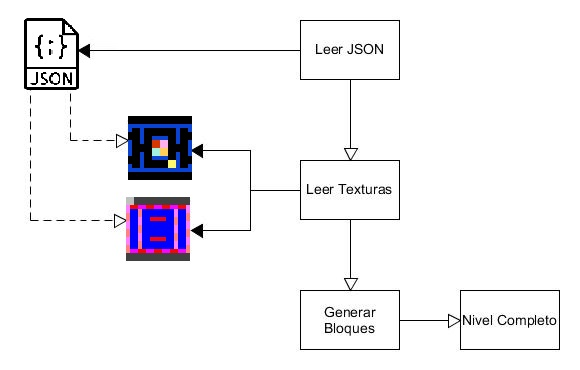
\includegraphics[width=0.7\textwidth]{images/estructura/escenas/level_generator}
	\centering
	\caption{Diagrama del proceso de generación de niveles}
	\label{generator_diagram}
\end{figure}

De esta forma es posible producir niveles rápidamente, los cuales son fáciles de modificar. La implementación del sistema es capaz de ignorar pequeños errores en el mapa, como asignación de colores a casillas vacías o la presencia de colores que no se corresponden con ningún tipo de ladrillos.

Por otra parte, el este sistema también limitaciones:
\begin{itemize}
  \item En primer lugar, solo una pequeña cantidad de colores pueden ser asignados a tipos de ladrillos. Esto se debe a las discrepancias entre los formatos de colores (los componentes RGB de los colores se guardan como enteros entre 0 y 255 en las texturas, pero como números de punto flotante entre 0 y 1 en la clase Color), la cual provoca perdida de información durante la conversión y nos fuerza a utilizar valores de color que sean fracciones exactas de 256. 
  \item En segundo lugar, se trata de un sistema poco escalable, permitiendo un tamaño único de campo de juego y poca capacidad para ``personalizar'' los tipos de bloque más allá de su color; por lo que sería necesario realizar cambios importantes en caso de que se necesitaran construir niveles más complejos
\end{itemize}

\section{Objetos}
El comportamiento de un videojuego desarrollado en Unity viene dado por los \textbf{objetos} que hay en el juego y las interacciones que existen entre estos. Estos objetos deben de poder influir en distintos dominios del código, como el rende rizado, el sonido o las físicas, lo cual puede causar un importante problema de acoplamiento entre clases. Para solucionar este problema, Unity hace uso del patrón de diseño \textbf{Component}. Este patrón de diseño  
consiste en aislar los distintos dominios en clases \textbf{componentes}, las cuales pueden ser asociadas a un objeto contenedor de componentes \cite{game_programming_patterns}.

La clase contenedor de componentes en Unity se llama \textbf{GameObjects}\footnote{https://docs.unity3d.com/ScriptReference/GameObject.html}. Los GameObjets se instancian mediante el editor de Unity o mediante código con el método estático \textbf{Instantiate}\footnote{https://docs.unity3d.com/ScriptReference/Object.Instantiate.html}. Estos objetos carecen de funcionalidad, a excepción de una serie de métodos para realizar busquedas entre los GameObjets de una escena. La funcionalidad de los GameObjects viene dada por los objetos de la clase \textbf{Component}\footnote{https://docs.unity3d.com/Manual/Components.html}. Esta clase es padre de multitud de componentes con diferente funcionalidad. Algunos de los componentes más importantes de Unity son los siguientes:
\begin{itemize}
\item \textbf{Transform}\footnote{https://docs.unity3d.com/ScriptReference/Transform.html}: Este componente almacena la posición, rotación y escala del objeto en la escena. Cada transform tiene un padre, lo que permite aplicar las transformaciones de forma jerárquica. Como su función es tan importante, todos los GameObjets tienen uno asociado.
\item \textbf{Collider}\footnote{https://docs.unity3d.com/ScriptReference/Collider.html}: Los colliders son una familia de componentes que permiten realizar la detección de colisiones. Existen muchos tipos de colliders dependiendo de su forma (BoxCollider, SphereCollider...). La clase Collider y sus hijos interaccionan con el motor de físicas 3D de Unity, para las colisiones entre objetos en 2D se utiliza la familia de clases \textbf{Collider2D}.
\item \textbf{Rigidbody}\footnote{https://docs.unity3d.com/ScriptReference/Rigidbody.html}: Esta clase se utiliza para la simulación física de cuerpos rígidos en 3D. Rigidbody contiene metodos para aplicar cambios de posición y rotación a objetos basándose en su velocidad, aceleración, fricción... Para objetos en 2D, existe una clase equivalente llamada \textbf{Rigidbody2D}.
\item \textbf{Renderer}\footnote{https://docs.unity3d.com/ScriptReference/Renderer.html}: Este componente permite renderizar modelos y texturas en la escena. 
\item \textbf{Audio Source}\footnote{https://docs.unity3d.com/ScriptReference/AudioSource.html}: Los audio source son componentes que permiten a los objetos emitir clips sonido. El componente permite aplicar transformaciones en tiempo real a los sonidos que emite, como modificar su volumen o la altura de su tono.
\item \textbf{Animator}\footnote{https://docs.unity3d.com/ScriptReference/Animator.html}: Este componente permite añadir animaciones a los objetos. Se trata de una máquina de estados finitos que reproduce clips de animación de forma condicional. Estos clips pueden producir variaciones en las propiedades de otros componentes del objeto en función del tiempo.
\item \textbf{Particle System}\footnote{https://docs.unity3d.com/ScriptReference/ParticleSystem.html}: Es un componente que emite \textbf{partículas}, pequeñas imágenes 2D que permiten crear efectos visuales como fuego o explosiones.
\end{itemize}

Aparte de los componentes incluidos en Unity, los desarrolladores pueden construir sus propios componentes y añadirlos a los GameObjets. La clase \textbf{MonoBehaviour}\footnote{https://docs.unity3d.com/ScriptReference/MonoBehaviour.html
} se utiliza como base para estos componentes, incluye una serie de métodos llamados \textbf{eventos} que son llamados automáticamente cuando se cumplen ciertas condiciones, como por ejemplo al principio de la ejecución (evento Start).

En los siguientes apartados contienen una descripción de los distintos objetos que forman el juego. Estas descripciones describen la función del objeto, jerarquía de GameObjects que lo forman, los Componentes que tienen asociados y el código de los scripts que definen su comportamiento.

\subsection{Personaje Principal}
El \textbf{personaje principal} es el avatar del jugador en el juego, al que controla directamente mediante el teclado. Su comportamiento es bastante sencillo: el personaje se mueve cuando el jugador pulsa las flechas de dirección, y crea una ``paleta'' cuando se pulsa la tecla espacio. Usando la paleta, el personaje es capaz de redirigir la pelota, pero si la pelota impacta contra el directamente se quedará aturdido unos segundos. La paleta solo permanece activa unos instantes, en los cuales el personaje permanece inmóvil, por lo que presenta un desafío para el jugador, que debe saber posicionarse correctamente. El personaje reproduce también una animación al inicio de los niveles y otra al final, en la que entra y sale de la sala del juego.

\begin{figure}[h]
	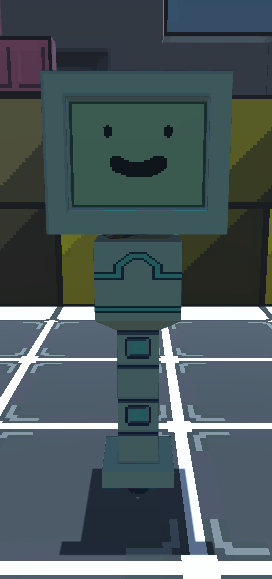
\includegraphics[width=0.30\textwidth]{images/estructura/fisica/flick_happy_small}
	\centering
	\caption{Modelo del personaje principal}
\end{figure}

Para la implementación del jugador se utilizan dos GameObjects anidados. El GameObject padre se encarga de la lógica del personaje mientras que el objeto hijo sirve para contener el modelo del personaje. La lógica del GameObject principal viene dada por una serie de componentes que tiene asociados: 
\begin{itemize}
	\item Un \textbf{Rigidbody} y un \textbf{Collider}. Estos componentes se encargan, respectivamente, de almacenar las propiedades físicas del personaje (velocidad, aceleración, gravedad...) y de realizar la detección de colisiones con otros objetos.
	\item Un \textbf{Audio Source}, el cual se encarga de reproducir los sonidos del personaje.
	\item Un \textbf{Animator}, el cual reproduce las animaciones del jugador. Las animaciones (realizadas en el propio editor de Unity) estar guardadas como ``clips'' que el Animator carga dependiendo del estado interno del personaje.
	\item Un \textbf{Script} de la clase \textbf{MainCharacter}, el cual se ocupa de recibir la información de entrada del jugador y coordinar las acciones del resto de componentes.
\end{itemize}

\begin{figure}[h]
	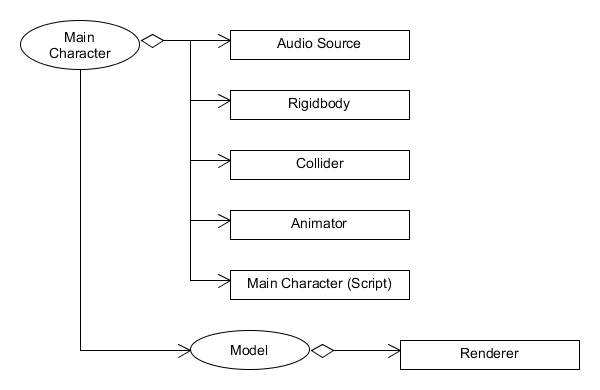
\includegraphics[width=0.8\textwidth]{images/estructura/objetos/main_character}
	\centering
	\caption{Diagrama de componentes del personaje principal.}
\end{figure}

El Script del personaje principal basa su funcionamiento en una \textbf{Maquina de Estados Finitos}. Los estados (Figura \ref{player}) que componen el comportamiento del personaje principal son los siguientes:
\begin{itemize}
	\item \textbf{Enter}: Es el estado inicial. En este estado el personaje, posicionado fuera de escena, se mueve hacia el interior de la sala hasta colocarse en el centro de esta. Durante este estado, la colisión y la gravedad están desactivadas, lo que le permite entrar en la sala cerrada. Una vez terminada la animación, pasa al estado \textbf{Stand}.
  	\item \textbf{Stand}: Se trata del estado principal. En él, el personaje espera inmóvil a recibir las órdenes del personaje. Si se pulsan las flechas de dirección, el personaje pasará al estado \textbf{Move} y si se pulsa la tecla espacio, se pasará al estado \textbf{Paddle}.
	\item \textbf{Move}: En este estado el personaje se mueve a velocidad constante en la dirección determinada por las flechas pulsadas. Cuando ninguna de las flechas de dirección esté siendo pulsadas, se volverá al estado \textbf{Stand}. En este estado también se puede pulsar la tecla espacio para moverse entrar en el estado \textbf{Paddle}.
	\item \textbf{Paddle}: En este estado el personaje crea frente a el un objeto Paleta que sirve para desviar la pelota. La paleta tiene un temporizador que hace que, al acabarse, la paleta desaparezca y el personaje vuelve al estado \textbf{Stand}. Durante este estado el jugador no se puede mover, aunque si se entró desde el estado \textbf{Move} todavía se conservará parte de la velocidad debido a la inercia.
	\item \textbf{Confused}: El personaje entra en este estado cuando la pelota le golpea, independientemente de en qué estado se encuentre. En este estado, el jugador girará aturdido durante unos instantes antes de volver al estado \textbf{Stand}, como penalización para el jugador por no haber golpeado la pelota correctamente.
	\item \textbf{Dead}: El personaje entra en este estado cuando la pelota es destruida, sin importar el estado anterior. En este estado el personaje se desploma derrotado y se queda inmóvil, a espera de la pantalla de ``fin del juego''.
    \item \textbf{Exit}: Cuando se completa un nivel, el personaje entra en este estado. El estado tiene dos partes: primero, el personaje permanece inmóvil a la espera de que la puerta del nivel se abra; y una vez esta esté abierta, el personaje avanza a través de ella hacia el siguiente nivel.
\end{itemize}

\begin{figure}[h]
	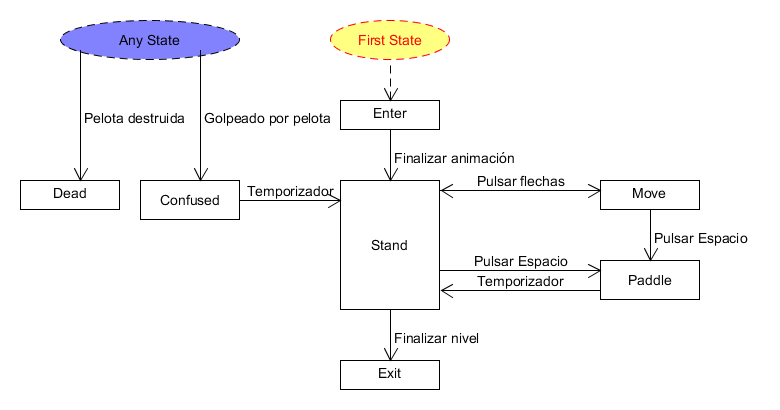
\includegraphics[width=0.95\textwidth]{images/estructura/fisica/player}
	\centering
	\caption{Diagrama de estados del personaje principal}
	\label{player}
\end{figure}

Una parte fundamental del comportamiento del personaje es su movimiento, presente en la mayor parte de los estados, tanto los controlados por el jugador (Move y Paddle) como los movimientos automáticos (las animaciones de Enter y Exit. Estos movimientos están implementados mediante el sistema de físicas, aplicándole al jugador una fuerza en la dirección en la que se desea que se mueva. Se utilizan fuerzas en lugar de modificar directamente el valor de velocidad del personaje para darle al movimiento una ligera aceleración inicial, que es mucho más agradable y natural para el jugador. La fuerza que utiliza para el movimiento es muy alta y va acompañada de un factor de fricción también elevado, lo que permitía controlar al personaje con precisión. Esto se combina con una reducción de la fricción en el estado \textbf{Paddle} para que el personaje conservase parte de su velocidad al sacar la paleta, que sirve para aumentar el margen de error del jugador a la hora de intentar golpear la pelota.

La \textbf{Paleta} que el jugador crea durante el estado \textbf{Paddle} es un GameObject con un Renderer y un Collider asociado. Este objeto esta guardado como un Prefab que el personaje instancia al principio del estado. Durante la instanciación, el personaje incluye a la paleta en su jerarquía de objetos, para que siga los movimientos del personaje. Al finalizar el estado, la instancia de la paleta es destruida.

\begin{figure}[h]
	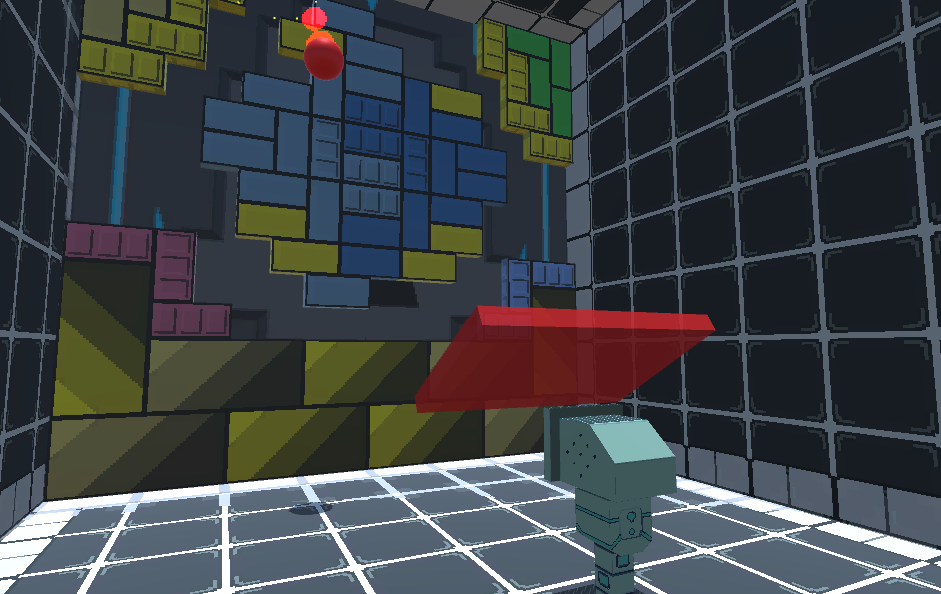
\includegraphics[width=0.8\textwidth]{images/estructura/fisica/flick_paddle}
	\centering
	\caption{Personaje principal activando la paleta}
\end{figure}

\subsection{Bola}
Podríamos considerar la pelota como el ''arma'' del personaje principal, el medio por el que el jugador interacciona con los objetos del juego. La pelota viaja en trayectoria rectilínea, rebotando en las paredes y el techo de la sala del juego. Al golpear la puerta, o los bloques que la cubren, estos reciben daño y la pelota rebota, pero si la pelota golpea el suelo de la sala es ella la que recibe daño, no el jugador. Si la pelota golpea el suelo tres veces, esta se destruye y partida se acaba. El jugador debe intentar golpear la pelota con la paleta para redirigiría hacia la puerta, evitando que toque el suelo.

\begin{figure}[h]
	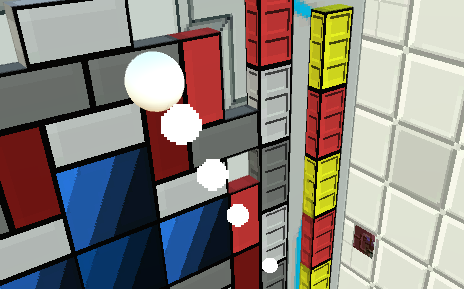
\includegraphics[width=0.65\textwidth]{images/estructura/fisica/ball_moving}
	\centering
	\caption{Pelota moviéndose}
\end{figure}

La pelota se compone de un único \textbf{GameObject}, el cual tiene una serie de componentes asociados:
\begin{itemize}
\item Un \textbf{Renderer}, el cual dibuja en pantalla el modelo de la bola.
\item Un \textbf{SphereCollider} para la detección de colisiones
\item Un \textbf{Rigidbody} para el control de movimiento.
\item Un \textbf{Audio Source} que emite los sonidos de impacto contra otros objetos.
\item Un \textbf{Animator} para ejecutar la animación de destrucción de la bola.
\item Un \textbf{Particle System} que se utiliza para producir varios efectos especiales.
\item Un \textbf{Script} de la clase \textbf{Ball} que controla el comportamiento de la bola, especialmente su reacción cuando colisiona con otros objetos.
\end{itemize}

\begin{figure}[h]
	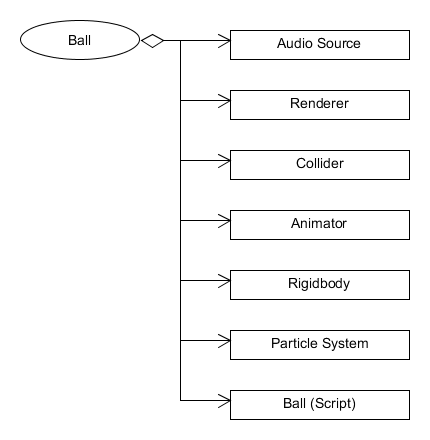
\includegraphics[width=0.65\textwidth]{images/estructura/objetos/ball}
	\centering
	\caption{Componentes del objeto Ball.}
\end{figure}

El script \textbf{Ball} basa su funcionamiento en una máquina de estados finitos al igual que el jugador; sin embargo, es significativamente más simple ya que cuenta solo con tres estados: \textbf{Normal} (su comportamiento normal de movimiento), \textbf{Destroy} (animación de destrucción de la pelota que se reproduce al final del juego) y \textbf{Locked} (estado especial en el que la pelota permanece quieta e invisible, para la cinemática de inicio y final del nivel). 

La complejidad de este script reside en la \textbf{tabla de interacciones} de la bola, debido a que la bola tiene una reacción distinta dependiendo de con que objeto del juego con el que colisione. Las posibles reacciones son:
\begin{itemize}
	\item Al golpear la \textbf{Puerta} de la sala o los \textbf{Bloques} que la cubren, estos sufrirán un punto de daño, y la pelota rebotará. Al iniciarse el rebote, la pelota empezará a caer en dirección al suelo de la sala.
	\item Al golpear las \textbf{Paredes} o el \textbf{Techo} de la sala, la pelota rebotará de forma natural.
	\item Al golpear el \textbf{Suelo} de la sala, la pelota recibirá un punto de daño. Además, la pelota rebotará, pero no de forma natural sino de forma que vaya en dirección a la puerta. Esto sirve principalmente para facilitar la tarea del jugador, ``regalándole'' un golpe a la puerta. La pelota también pierde la fuerza de la gravedad.
	\item Al golpear al \textbf{jugador}, este se quedará aturdido unos instantes y la pelota rebotará de forma natural.
	\item Al golpear la paleta del jugador, la pelota rebotará y perderá la fuerza de la gravedad. La dirección en la que rebotará la pelota dependerá del punto de la paleta en el que golpeó la pelota, siendo la dirección normal al plano de la paleta si se golpea justo en el centro.
\end{itemize}
\begin{figure}[!htb]
   \begin{minipage}{0.5\textwidth}
     \centering
     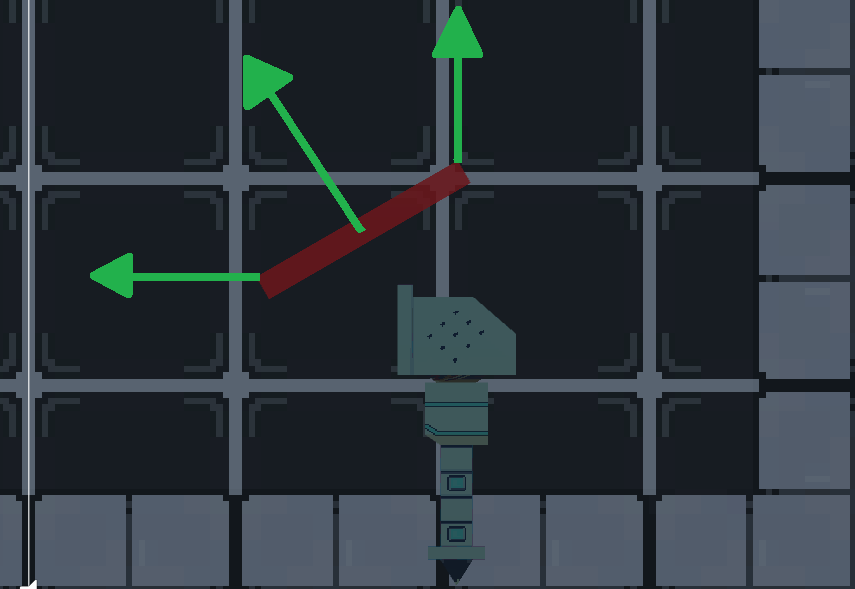
\includegraphics[width=0.9\linewidth, right]{images/estructura/fisica/paddle_direction_side}
   \end{minipage}\hfill
   \begin {minipage}{0.5\textwidth}
     \centering
     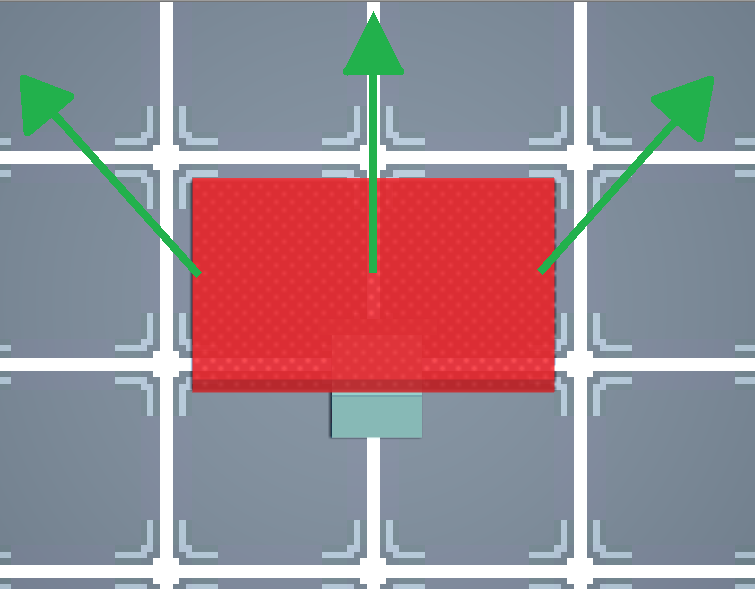
\includegraphics[width=0.9\linewidth, left]{images/estructura/fisica/paddle_direction_top}
   \end{minipage}
   \caption{Direcciones que tomaría la pelota dependiendo del punto de la paleta que golpee (Aproximada)}
\end{figure}
El movimiento de la pelota se basa íntegramente el motor de físicas de Unity. Al entrar en su estado \textbf{Normal}, la pelota recibe un impulso en una dirección dada y a partir de ahí se moverá sin fricción   de forma perpetua. Los movimientos ``antinaturales'' mencionados, el cambio de dirección al golpear el suelo o la paleta se realizan cambiando el vector de la velocidad de la pelota por un vector nuevo generado manualmente por código.

Aunque la pelota no tiene animación en si misma, a su comportamiento se le han añadido unos efectos de partículas, que sirven tanto para embellecer el juego como para crear guías visuales para el jugador. La pelota cuenta con tres efectos animados de partículas: una \textbf{``cola''} que marca la trayectoria que siguió la bola; un efecto circular que aparece cuando la bola \textbf{colisiona con las paredes}, el techo y el suelo, que sirven para marcar el punto de impacto de la bola y un efecto de \textbf{explosión final}. La trayectoria se produce mediante el componente \textbf{Particle System} de la pelota, pero para el efecto de impacto y explosión se hace uso de objetos externos, los cuales son instanciados, producen sus partículas y se eliminan automáticamente.
\begin{figure}[!htb]
   \begin{minipage}{0.48\textwidth}
     \centering
     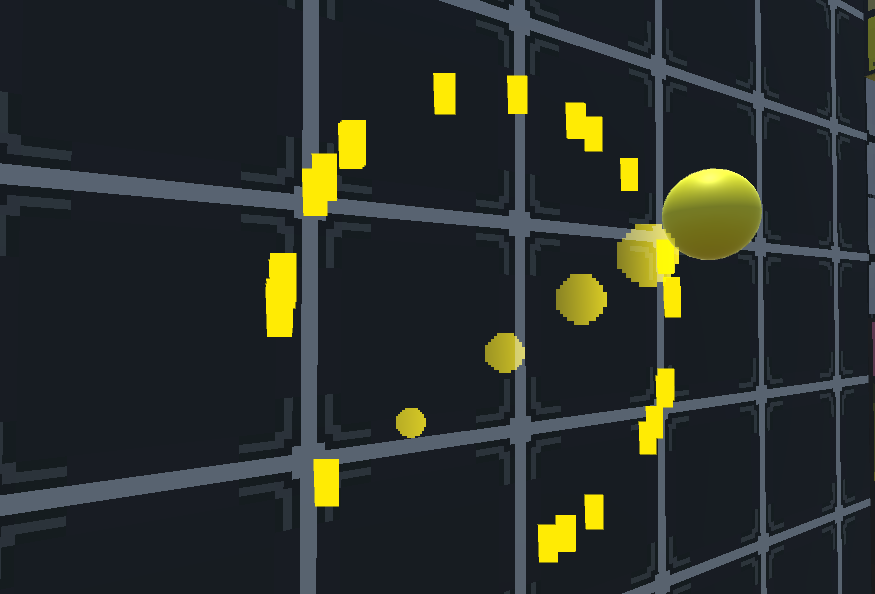
\includegraphics[width=0.7\linewidth, right]{images/estructura/fisica/ball_hit}
   \end{minipage}\hfill
   \begin {minipage}{0.48\textwidth}
     \centering
     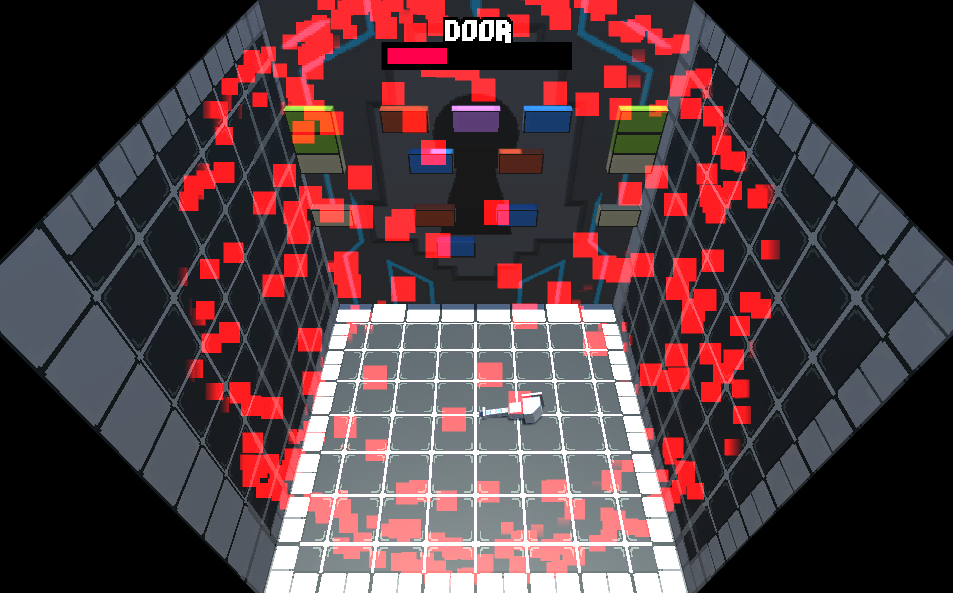
\includegraphics[width=0.7\linewidth, left]{images/estructura/objetos/ball_explosion}
   \end{minipage}
   \caption{Efectos de partículas: impacto en muro (izquierda) y explosión (derecha)}
\end{figure}

\subsection{Ladrillos}
Los ladrillos son el principal obstaculo del juego, ya que protegen la puerta de los golpes de la bola. Cada vez que la pelota golpea un ladrillo, este pierde un punto de vida. Cuando sus puntos de vida llegan a cero, el ladrillo se destruye. Los ladrillos se colocan delante de la puerta, en una \textbf{cuadricula} de 16 X 16 casillas. Cada nivel del juego tiene una configuración de ladrillos diferente. Para darle variedad al juego, existen varios tipos de ladrillos:
\begin{itemize}
\item \textbf{Ladrillo básico}: Es el ladrillo básico. Solo tiene un punto de vida. Este ladrillo mide 1 X 2 casillas.
\item \textbf{Ladrillo Multi-golpe}: Este ladrillo tiene tres puntos de vida, por lo que es más difícil romperlo. La textura de este ladrillo cambia con cada golpe para mostrar el daño infligido. Este ladrillo mide 1 X 2 casillas.
\item \textbf{Ladrillo Divisible}: Es un ladrillo de gran tamaño, mide 2 X 2 casillas. Aunque solo tiene un punto de vida, al romperse genera 4 ladrillos pequeños de 1 X 1 casillas de tamaño.
\item \textbf{Ladrillo Pequeño}: es un ladrillo idéntico al básico, salvo porque solo mide 1 X 1 casillas. Solo aparecen como resultado de la rotura de un ladrillo divisible.
\item \textbf{Ladrillo Irrompible}: Como su nombre indica, este ladrillo no puede ser destruido por la pelota. Miden 2 X 3 Casillas.
\end{itemize}

\begin{figure}[h]
	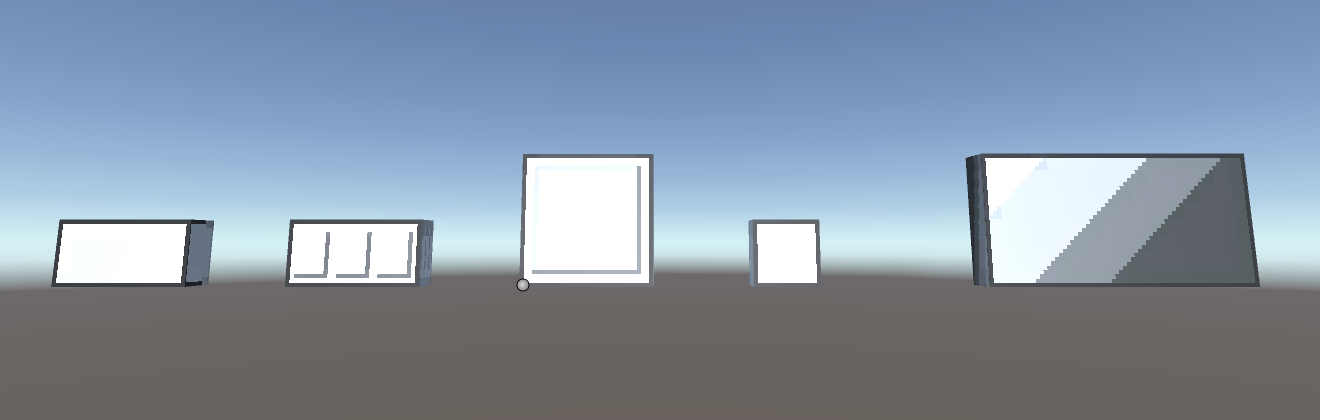
\includegraphics[width=0.65\textwidth]{images/estructura/objetos/brick_examples}
	\centering
	\caption{Modelos de los ladrillos}
\end{figure}

Independientemente de su comportamiento, cada ladrillo puede tener asignado un \textbf{color}. Esto permite dar variedad a los niveles y además hacerlos más memorables haciendo dibujos con los ladrillos.

Para implementar los ladrillos se utilizan dos GameObjects anidados. El primer GameObject se encarga de dotar al ladrillo de funcionalidad, mientras que el segundo contiene el modelo 3D del mismo. Los componentes que contienen los ladrillos son los siguientes: 
\begin{itemize}
\item Un \textbf{BoxCollider}, para la detección de colisiones.
\item Un \textbf{Particle System}, para la animación de destrucción.
\item Un \ un script de clase \textbf{Brick}, que contiene la funcionalidad del ladrillo.
\end{itemize}

\begin{figure}[h]
	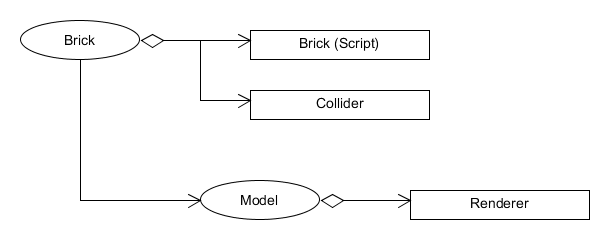
\includegraphics[width=0.65\textwidth]{images/estructura/objetos/bricks}
	\centering
	\caption{Componentes del objeto Brick.}
\end{figure}

El método principal de \textbf{Brick} se llama \textbf{DoDamamge}. Este método recibe como parámetro una cantidad de ``puntos de daño'' la cual sustrae a los puntos de vida actuales del ladrillo. Este método también destruye los ladrillos que han perdido todos sus puntos de vida y emite partículas del color del ladrillo con cada golpe recibido. Este sería el comportamiento de los ladrillos básicos, para programar los comportamientos específicos de los distintos tipos de ladrillos otros scripts que la funcionalidad de la clase \textbf{Brick}.

El cambio de textura de los ladrillos multigolpe está programado en la clase \textbf{TextureChangeBrick}, en la cual un se añade código adicional al método \textbf{DoDamage} para cambiar la textura del ladrillo de entre las presentes en una lista. El comportamiento del bloque divisible está en la clase \textbf{DivisibleBrick}, en la que durante la destrucción del ladrillo se instancian los cuatro ladrillos pequeños (que son ladrillos básicos pero con un modelo más pequeño. El script \textbf{UnbreakableBrick} es el que usan los ladrillos irrompibles, y en el el método \textbf{DoDamage} está vacío.

Todos estos ladrillos se guardan como prefabs entre los assets del juego, para que el generador de niveles los pueda instanciar.

\begin{figure}[h]
	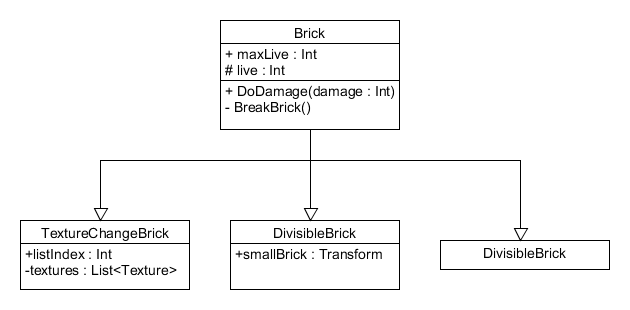
\includegraphics[width=0.65\textwidth]{images/estructura/objetos/brick_classes}
	\centering
	\caption{Jerarquía de clases.}
\end{figure}

\subsection{Sala y Puerta}
La \textbf{sala} es el entorno donde transcurre la acción del juego. Se trata de una habitación cúbica con una puerta cerrada en una de sus paredes. Frente a la puerta hay un muro formado por ladrillos cuya distribución cambia dependiendo del nivel. La puerta reacciona a los golpes con la pelota, moviéndose y perdiendo ``vida'' con cada golpe. Cuando la vida de la puerta llega a cero, la puerta se abre y el jugador avanza al siguiente nivel.

\begin{figure}[h]
	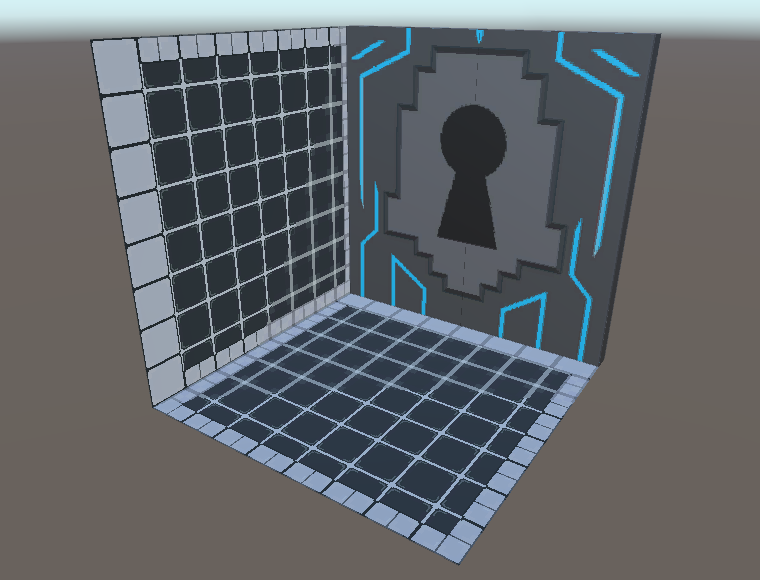
\includegraphics[width=0.8\textwidth]{images/estructura/objetos/captura_sala}
	\centering
	\caption{Sala vista desde el editor.}
\end{figure}

La implementación de la sala se basa en una combinación de GameObjects agrupados de forma jerárquica. Esto permite añadir funcionalidad diferente a los distintos elementos que conforman la sala. Los GameObjects son:
\begin{itemize}
\item \textbf{Room}: Es el objeto principal o ``padre'' que contiene a los demás. Contiene tres componentes: un \textbf{Audio Source}, el script \textbf{LevelGenerator} y el script \textbf{Room}.
\item \textbf{Walls}: Se trata de cuatro rectángulos que forman las tres paredes de la sala y el techo (que es funcionalmente idéntico a las paredes). Estos GameObjets tienen dos componentes: Un \textbf{MeshCollider} y un \textbf{Renderer}.
\item \textbf{Floor}: El suelo de la sala es similar a las paredes (un GameObject con un \textbf{MeshCollider} y un \textbf{Renderer}), pero está marcado de forma diferente para activar un comportamiento distinto en la pelota.
\item \textbf{Door}: La puerta de la sala ocupa la pared norte de la sala. Este GameObject tiene asociados tres componentes: un \textbf{BoxCollider}, un \textbf{Animator} y un script de clase \textbf{Door}. Anidados, la puerta contiene dos objetos \textbf{panel} independientes.
\end{itemize}

\begin{figure}[h]
	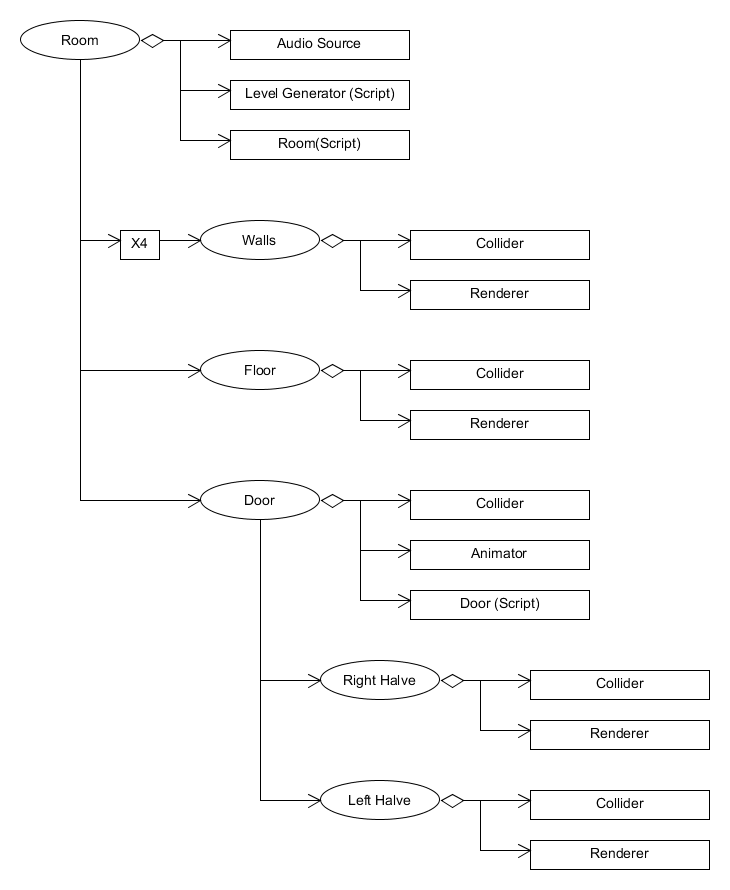
\includegraphics[width=0.8\textwidth]{images/estructura/objetos/room}
	\centering
	\caption{Diagrama de componentes de la sala.}
\end{figure}

Los dos scripts con los que cuenta la sala cumplen dos funciones muy distintas. \textbf{LevelGenerator} contiene el código responsable de la generación de niveles tal y como se describió en el apartado \ref{level_generator}. El script \textbf{Room}, por otro lado, se encarga de la gestión del estado de la sala.

Durante la ejecución del juego tienen lugar diversos eventos que deben producirse en un orden determinado. Estos eventos son producidos por diversos scripts asociados a GameObjects diferentes. El script \textbf{Room} sirve como intermediario entre los diversos objetos, recibiendo los mensajes producidos en los eventos y reenviándolos a los scripts que se encargan de iniciar los eventos siguientes. Dado la simplicidad de la secuencia de eventos, el sistema de mensajes se implementa mediante una serie de funciones públicas en el script \textbf{Room}.

La secuencia de eventos del juego puede agruparse en las siguientes etapas:
\begin{enumerate}
\item \textbf{Preambulo}: Es la secuencia de eventos anterior a que el jugador tome el control del juego. Los eventos de los que consta son los siguientes:
\begin{enumerate}
\item \textbf{Generación del nivel}: Cuando la escena se carga, el script \textbf{Room} llama a \textbf{LevelGenerator} y le suministra el índice del nivel que debe generarse.
\item \textbf{Entrada del jugador}: Simultáneamente a la carga del nivel, el \textbf{Personaje Principal} avanza desde fuera de la sala a su interior a través de la pared sur. El jugador llama a la sala cuando alcanza el centro de esta.
\item \textbf{Entrada del jefe}: Si se trata de un nivel de jefe, el jefe comienza su entrada en la sala. Al igual que el jugador, el jefe llama a la sala una vez su animación ha terminado.
\item \textbf{Activación de la pelota}: Una vez que el jugador (y el jefe) han entrado en la sala, la pelota se activa, haciendose visible en el centro de la sala. 
\item \textbf{Control del jugador}: Al mismo tiempo que se activa la pelota, el personaje principal empieza a reaccionar a las órdenes del jugador comienza el juego.
\end{enumerate}
\item \textbf{Juego}: En esta etapa de la ejecución, el jugador tiene control sobre el personaje principal. La etapa acaba cuando la puerta se queda sin vidas (lo que inicia la etapa de \textbf{Victoria}) o cuando la pelota toca el suelo tres veces (lo que inicia la etapa de \textbf{Derrota}).
\item \textbf{Victoria}: Cuando el jugador supera un nivel, se sucede la siguiente secuencia de eventos:
\begin{enumerate}
\item \textbf{Ocultar pelota}: Se envía un mensaje a la pelota para detener su movimiento y desactivar tanto su collider como su renderer, provocando que la pelota se vuelva invisible e intangible.
\item \textbf{Animación de la puerta}: Al mismo tiempo que se desactiva la pelota, se envía un mensaje a la puerta para que empiece su animación de apertura.
\item \textbf{Romper los ladrillos}: Cuando acaba la animación de la puerta, esta manda un mensaje a todos sus ladrillos para que se destruyan.
\item \textbf{Salida del personaje principal}: Una vez finalizada la animación de la puerta, se envía un mensaje al personaje principal para que salga de la sala por la puerta.
\item \textbf{Cambio de escena}: Cuando el personaje principal se ha alejado lo suficiente de la sala comienza el cambio de escena. Si se trataba del ultimo nivel, se carga la \textbf{escena de victoria}, si no, se vuelve a cargar la escena de juego, incrementando el índice de nivel.
\end{enumerate}
\item \textbf{Derrota}: La secuencia de acciones que ocurren cuando el jugador pierde el juego son las siguientes:
\begin{enumerate}
\item \textbf{Destrucción de la Pelota}: Se envía un mensaje a la pelota, que comienza su animación de destrucción.
\item \textbf{Derrota del jugador}: Cuando la pelota acaba su animación, se envía un mensaje al jugador para que comience con su animación de derrota.
\item \textbf{Cambio de escena}: Un tiempo después del final de la animación del jugador, se inicia el cambio de escena a \textbf{la escena de fin del juego}.
\end{enumerate}
\end{enumerate}

El comportamiento de la \textbf{Puerta} es independiente de el de la sala. La funcion de su script, \textbf{Door}, es la de detectar la colisión de la pelota con la puerta para así reducir los puntos de vida de esta e iniciar el final del nivel si los puntos de vida llegan a cero.

\subsection{Jefe}
Un \textbf{jefe final}, o monstruo jefe, es un enemigo poderoso al que los jugadores deben enfrentarse para poder alcanzar algún objetivo dentro del juego \cite{game_design_patterns}. Los jefes sirven principalmente para tres propósitos: dar clausura a una sección del juego, al colocarse al final de una sección, nivel o fase; ofrecen variedad al juego, al suponer una variación con respecto al juego corriente y finalmente sirven como ``test'' para el jugador, al tratarse de un desafió mucho mayor que los anteriores. 

Para este juego, el jefe final es el único ``enemigo'' al que se enfrenta el jugador, que aparece en el nivel 11 del juego. Este jefe se comporta como un \textbf{``clon''} o ``rival'' del jugador: su objetivo es impedir que la pelota golpee la puerta, moviéndose y redirigiéndola de forma similar a como lo haría el jugador. La forma de derrotar a este jefe es idéntica de a como se supera cualquier fase: Golpeando la puerta suficientes veces. 

El jefe se mueve a \textbf{velocidad constante}, siempre pegado a la pared, intentando bloquear la pelota. Sin embargo, si detuviese siempre la pelota, sería un desafío imposible de superar, lo que no sería divertido para el jugador. La idea es que este jefe se juegue como si de una partida de tenis se tratase, con dos adversarios intercambiándose la pelota hasta que uno de los dos falle. Por ello, el jefe tendrá un \textbf{sistema de energía} que determinara su eficiencia a la hora de jugar e ira consumiéndose según avance la partida.

\begin{figure}[h]
	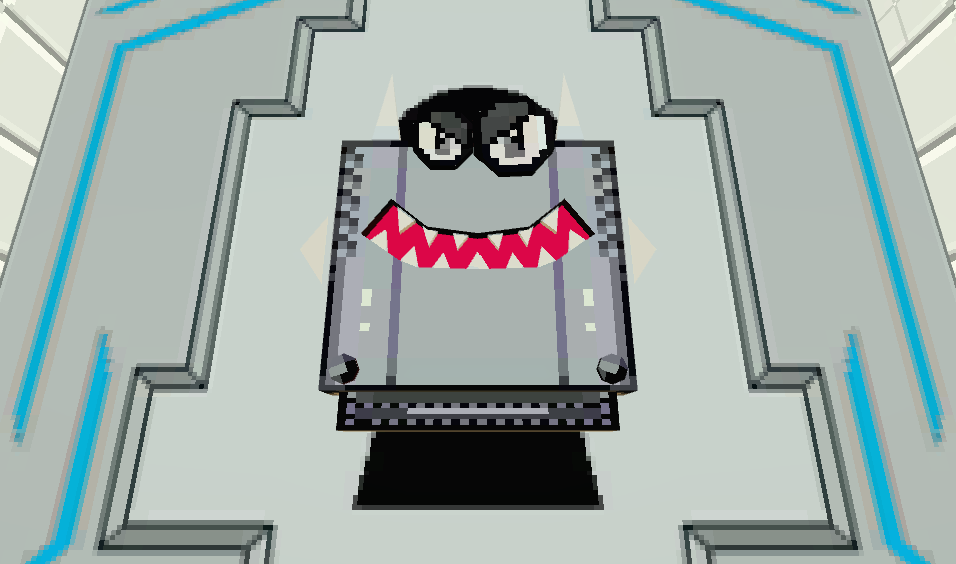
\includegraphics[width=0.30\textwidth]{images/estructura/jefe/boss-captura}
	\centering
	\caption{Modelo del Jefe.}
\end{figure}

La implementación del jefe utiliza \textbf{dos GameObjects anidados}. El GameObject principal contiene los componentes necesarios para el funcionamiento del jefe, mientras que el GameObject anidado contiene el modelo de este. Los componentes del GamObject padre son los siguientes:
 \begin{itemize}
	\item \textbf{RigidBody}: Este componente almacena las propiedades físicas del jefe, como su velocidad o aceleración.
	\item \textbf{Collider}: Este componente permite realizar la detección de colisiones entre el jefe y otros objetos.
	\item \textbf{Animator}: Permite añadir animaciones al GameObject, las cuales alteran las propiedades de sus componentes basándose en el tiempo. Se utiliza para crear dotar al jefe de animaciones sencillas de modo que no resulte demasiado estático.
	\item \textbf{Audio Source}: Sirve para emitir sonidos y música. El jefe lo utiliza para emitir sonidos en situaciones concretas, como al golpear la pelota o al ser derrotado.
	\item Dos \textbf{Scripts} que controlan el comportamiento del jefe: \textbf{BossController} y \textbf{BossAI}.
\end{itemize}

\begin{figure}[h]
	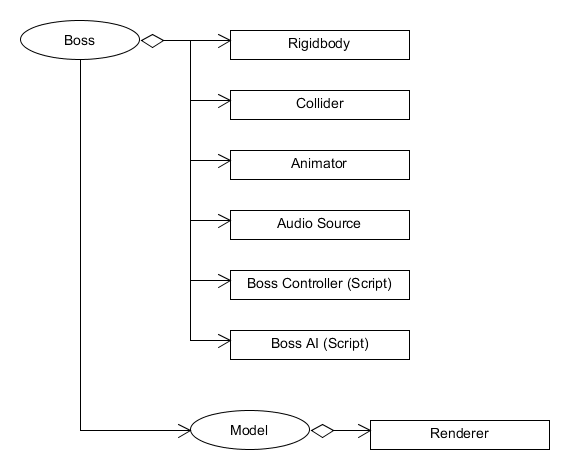
\includegraphics[width=0.8\textwidth]{images/estructura/objetos/boss}
	\centering
	\caption{Diagrama de componentes del jefe.}
\end{figure}

El comportamiento del jefe se encuentra dividido en dos scripts para separar las acciones que puede realizar el jefe de la inteligencia artificial que determina cuales de esas acciones debe realizar. Los dos scripts implementan el patrón de diseño \textbf{Strategy}\cite{libro_esi}.

\textbf{BossController} contiene la información y las funciones necesarias para facilitar el movimiento del jefe. El método principal de esta clase, \textit{MoveDirection()}, permite mover al jefe a velocidad constante en el ángulo suministrado como parámetro, siempre de forma paralela al plano de la puerta. El movimiento se implementa a través del componente Rigidbody, aplicando fuerza constante en la dirección indicada, lo que crea un movimiento con una ligera aceleración que resulta más natura que un cambio instantáneo de velocidad. 

El script implementa cambien el sistema de energía. El jefe tiene una variable que determina la cantidad de \textbf{energia} que tiene el jefe, la cual se utiliza para calcular la velocidad de su movimiento: cuanta más energía, más rápido es el movimiento. La energía baja cada vez que la pelota golpea al jefe e incrementa cuando golpea la puerta.

El segundo script, \textbf{BossAI}, implementa la inteligencia artificial del jefe. El script se encarga de determinar determinar cuándo y en qué dirección debe moverse, que animación debe reproducirse y cuando reproducir los efectos de sonido. La implementación de este comportamiento se realiza mediante una \textbf{Máquina de Estados Finitos}. Los estados de los que se compone son los siguientes:
 \begin{itemize}
	\item \textbf{Out}: El jefe espera fuera del área de juego, inmóvil, a la espera de la entrada del jugador en la sala.
	\item \textbf{Intro}: El jefe se mueve a su posición inicial y realiza su animación inicial. Este movimiento se implementa mediante el uso de animaciones en lugar de mediante el BossController dado que debe atravesar las paredes de la sala.
	\item \textbf{Wait}: En este estado, el jefe permanece inmóvil a la espera de un estímulo que le haga cambiar iniciar el movimiento, en concreto, que se detecte que la pelota se aproxima a la puerta.
	\item \textbf{Move}: El jefe se mueve en dirección a la pelota utilizando los métodos de BossController. El movimiento se detendrá si se consigue golpear la pelota o si la pelota golpea la puerta. 
	\item \textbf{Hurt}: En este estado el jefe permanece inmóvil mientras se reproduce una animación de daño. Tras esta breve pausa, el jefe retorna al estado Wait.
	\item \textbf{Death}: Cuando la puerta se abre, el jefe realiza una animación de destrucción, en la que el jefe se vuelve invisible y emite una explosión de partículas. 
\end{itemize}

\begin{figure}[h]
	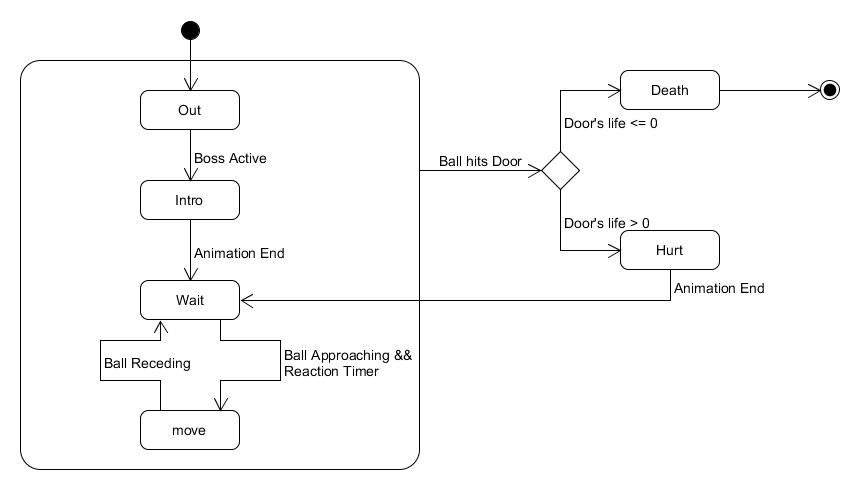
\includegraphics[width=1\textwidth]{images/estructura/jefe/boss-estados}
	\centering
	\caption{Diagrama de estados del jefe.}
\end{figure}
